% Options for packages loaded elsewhere
\PassOptionsToPackage{unicode}{hyperref}
\PassOptionsToPackage{hyphens}{url}
%
\documentclass[
]{article}
\usepackage{amsmath,amssymb}
\usepackage{iftex}
\ifPDFTeX
  \usepackage[T1]{fontenc}
  \usepackage[utf8]{inputenc}
  \usepackage{textcomp} % provide euro and other symbols
\else % if luatex or xetex
  \usepackage{unicode-math} % this also loads fontspec
  \defaultfontfeatures{Scale=MatchLowercase}
  \defaultfontfeatures[\rmfamily]{Ligatures=TeX,Scale=1}
\fi
\usepackage{lmodern}
\ifPDFTeX\else
  % xetex/luatex font selection
\fi
% Use upquote if available, for straight quotes in verbatim environments
\IfFileExists{upquote.sty}{\usepackage{upquote}}{}
\IfFileExists{microtype.sty}{% use microtype if available
  \usepackage[]{microtype}
  \UseMicrotypeSet[protrusion]{basicmath} % disable protrusion for tt fonts
}{}
\makeatletter
\@ifundefined{KOMAClassName}{% if non-KOMA class
  \IfFileExists{parskip.sty}{%
    \usepackage{parskip}
  }{% else
    \setlength{\parindent}{0pt}
    \setlength{\parskip}{6pt plus 2pt minus 1pt}}
}{% if KOMA class
  \KOMAoptions{parskip=half}}
\makeatother
\usepackage{xcolor}
\usepackage[margin=1in]{geometry}
\usepackage{longtable,booktabs,array}
\usepackage{calc} % for calculating minipage widths
% Correct order of tables after \paragraph or \subparagraph
\usepackage{etoolbox}
\makeatletter
\patchcmd\longtable{\par}{\if@noskipsec\mbox{}\fi\par}{}{}
\makeatother
% Allow footnotes in longtable head/foot
\IfFileExists{footnotehyper.sty}{\usepackage{footnotehyper}}{\usepackage{footnote}}
\makesavenoteenv{longtable}
\usepackage{graphicx}
\makeatletter
\def\maxwidth{\ifdim\Gin@nat@width>\linewidth\linewidth\else\Gin@nat@width\fi}
\def\maxheight{\ifdim\Gin@nat@height>\textheight\textheight\else\Gin@nat@height\fi}
\makeatother
% Scale images if necessary, so that they will not overflow the page
% margins by default, and it is still possible to overwrite the defaults
% using explicit options in \includegraphics[width, height, ...]{}
\setkeys{Gin}{width=\maxwidth,height=\maxheight,keepaspectratio}
% Set default figure placement to htbp
\makeatletter
\def\fps@figure{htbp}
\makeatother
\setlength{\emergencystretch}{3em} % prevent overfull lines
\providecommand{\tightlist}{%
  \setlength{\itemsep}{0pt}\setlength{\parskip}{0pt}}
\setcounter{secnumdepth}{5}
\newlength{\cslhangindent}
\setlength{\cslhangindent}{1.5em}
\newlength{\csllabelwidth}
\setlength{\csllabelwidth}{3em}
\newlength{\cslentryspacingunit} % times entry-spacing
\setlength{\cslentryspacingunit}{\parskip}
\newenvironment{CSLReferences}[2] % #1 hanging-ident, #2 entry spacing
 {% don't indent paragraphs
  \setlength{\parindent}{0pt}
  % turn on hanging indent if param 1 is 1
  \ifodd #1
  \let\oldpar\par
  \def\par{\hangindent=\cslhangindent\oldpar}
  \fi
  % set entry spacing
  \setlength{\parskip}{#2\cslentryspacingunit}
 }%
 {}
\usepackage{calc}
\newcommand{\CSLBlock}[1]{#1\hfill\break}
\newcommand{\CSLLeftMargin}[1]{\parbox[t]{\csllabelwidth}{#1}}
\newcommand{\CSLRightInline}[1]{\parbox[t]{\linewidth - \csllabelwidth}{#1}\break}
\newcommand{\CSLIndent}[1]{\hspace{\cslhangindent}#1}
\usepackage{tocbibind}
\usepackage{setspace}\doublespacing
\usepackage{indentfirst}\setlength\parindent{24pt}
\usepackage{float}
\usepackage{float} \floatplacement{figure}{H}
\usepackage{caption}
\pagenumbering{gobble}
\newcommand{\chapterone}{\setcounter{table}{0}
\renewcommand{\thetable}{1.\arabic{table}}
\setcounter{figure}{0}
\renewcommand{\thefigure}{1.\arabic{figure}}}
\newcommand{\beginsupplementAone}{\setcounter{table}{0}
\renewcommand{\thetable}{A1.\arabic{table}}
\setcounter{figure}{0}
\renewcommand{\thefigure}{A1.\arabic{figure}}}
\usepackage{booktabs}
\usepackage{longtable}
\usepackage{array}
\usepackage{multirow}
\usepackage{wrapfig}
\usepackage{float}
\usepackage{colortbl}
\usepackage{pdflscape}
\usepackage{tabu}
\usepackage{threeparttable}
\usepackage{threeparttablex}
\usepackage[normalem]{ulem}
\usepackage{makecell}
\usepackage{xcolor}
\ifLuaTeX
  \usepackage{selnolig}  % disable illegal ligatures
\fi
\IfFileExists{bookmark.sty}{\usepackage{bookmark}}{\usepackage{hyperref}}
\IfFileExists{xurl.sty}{\usepackage{xurl}}{} % add URL line breaks if available
\urlstyle{same}
\hypersetup{
  hidelinks,
  pdfcreator={LaTeX via pandoc}}

\author{}
\date{\vspace{-2.5em}}

\begin{document}

\begin{centering} 

\Huge
{\bf This is the title of the thesis. The command bf allows to set it to bold. Huge sets it to the maximal size}

\vspace{5cm}
\huge
{Full Name}

\LARGE
{Doctor of Philosophy}

\vspace{-0.5cm}
\LARGE
{in Cognitive Neuroscience and Neuroimaging or Psychology}

\vspace{4cm}
\LARGE
{University of York}

\vspace{-0.5cm}
\LARGE
{Psychology}

\vspace{1cm}
\LARGE
{Month and year of submission}

\end{centering}

\pagebreak

\pagenumbering{arabic}
\setcounter{page}{2}

\hypertarget{abstract}{%
\section*{Abstract}\label{abstract}}
\addcontentsline{toc}{section}{Abstract}

\pagebreak

\setcounter{tocdepth}{5}
\tableofcontents
\pagebreak
\listoffigures
\pagebreak
\listoftables

\pagebreak

\hypertarget{acknowledgements}{%
\section*{Acknowledgements}\label{acknowledgements}}
\addcontentsline{toc}{section}{Acknowledgements}

\pagebreak

\hypertarget{authors-declaration}{%
\section*{Author's Declaration}\label{authors-declaration}}
\addcontentsline{toc}{section}{Author's Declaration}

\pagebreak

\hypertarget{supervisors-statement}{%
\section*{Supervisor's Statement}\label{supervisors-statement}}
\addcontentsline{toc}{section}{Supervisor's Statement}

\pagebreak
\chapterone

\hypertarget{chapter-1-title-of-the-chapter}{%
\section{Chapter 1: Title of the chapter}\label{chapter-1-title-of-the-chapter}}

\hypertarget{section-title}{%
\subsection{Section title}\label{section-title}}

We write some text here.

To start a new paragraph, you need to leave a blank line between the previous paragraph and the new paragraph.

You might need to include footnotes.\footnote{This is how you include a footnote. The text within the square brackets will appear in the footnote.}

\begin{quote}
You might want to indent an entire paragraph and not only the first: by using the `\textgreater{}' symbol, the entire paragraph will be indented. The size of the indentadion is determined by the parindent\{\} command in the header-includes section at the beginning.
\end{quote}

\hypertarget{subsection-title}{%
\subsubsection{Subsection title}\label{subsection-title}}

Some more text here.

\hypertarget{subsection-level-4-no-hspace}{%
\paragraph{Subsection level 4 no hspace}\label{subsection-level-4-no-hspace}}

R markdown works perfectly up to the third level of section numbering. From the fourth, however, it is not able to format correctly and writes this sentence next to the subsection title, as shown by this sentence. To stop it from doing this, we use the ``hspace'' command (an example is shown in the next section).

\hypertarget{subsection-level-4-hspace}{%
\paragraph{Subsection level 4 hspace}\label{subsection-level-4-hspace}}

\hspace{-2.5em}

Hspace places the new paragraph on a new line.

\hypertarget{subsection-level-5}{%
\subparagraph{Subsection level 5}\label{subsection-level-5}}

\hspace{-2.5em}

Here is an example of how to write an equation:

\begin{equation}
\label{eq:example}
B = \sqrt{R^2+L^2},
\end{equation}

\noindent Using ``noindent'' allows you to remove the initial indent for this paragraph.

By using the following command, you can refer to your figure and R markdown will keep the count automatically: see example in Figure \ref{fig:examplefig1}. Additionally, R markdown creates hyperlinks to figures, tables and references, so that, if you click on them, it will take you directly to the figure, table or reference within the reference list. Figures and tables are automatically added to your LoF and LoT.

There are different ways to reference. To include a reference, use the cite key of the reference. I would suggest to format the cite key as @AuthorDate, so this is what it looks like: Author (\protect\hyperlink{ref-Author2023}{2023}). As you can see, the reference in the PDF appears as Author (date). To have the reference appear as (Author, date), use square brackets: (\protect\hyperlink{ref-Author2023}{Author, 2023}). In APA style, if two references have the same authors, R markdown will write them as (Author, date1; date2) automatically: (\protect\hyperlink{ref-Author2024}{Author, 2024}, \protect\hyperlink{ref-Author2023}{2023}). To include more references within one square bracket, use a semicolon: (\protect\hyperlink{ref-Author2024}{Author, 2024}, \protect\hyperlink{ref-Author2023}{2023}; \protect\hyperlink{ref-Author2025}{Author and Authortwo, 2025}). You can also include some text within a square bracket and a reference. Make sure to use a semicolon between the references if you include multiple ones: (\protect\hyperlink{ref-Author2026}{Author et al., 2026}; here is an example, \protect\hyperlink{ref-Author2025}{Author and Authortwo, 2025}). Markdown will automatically compile the reference list at the end of the document.

\begin{figure}

{\centering 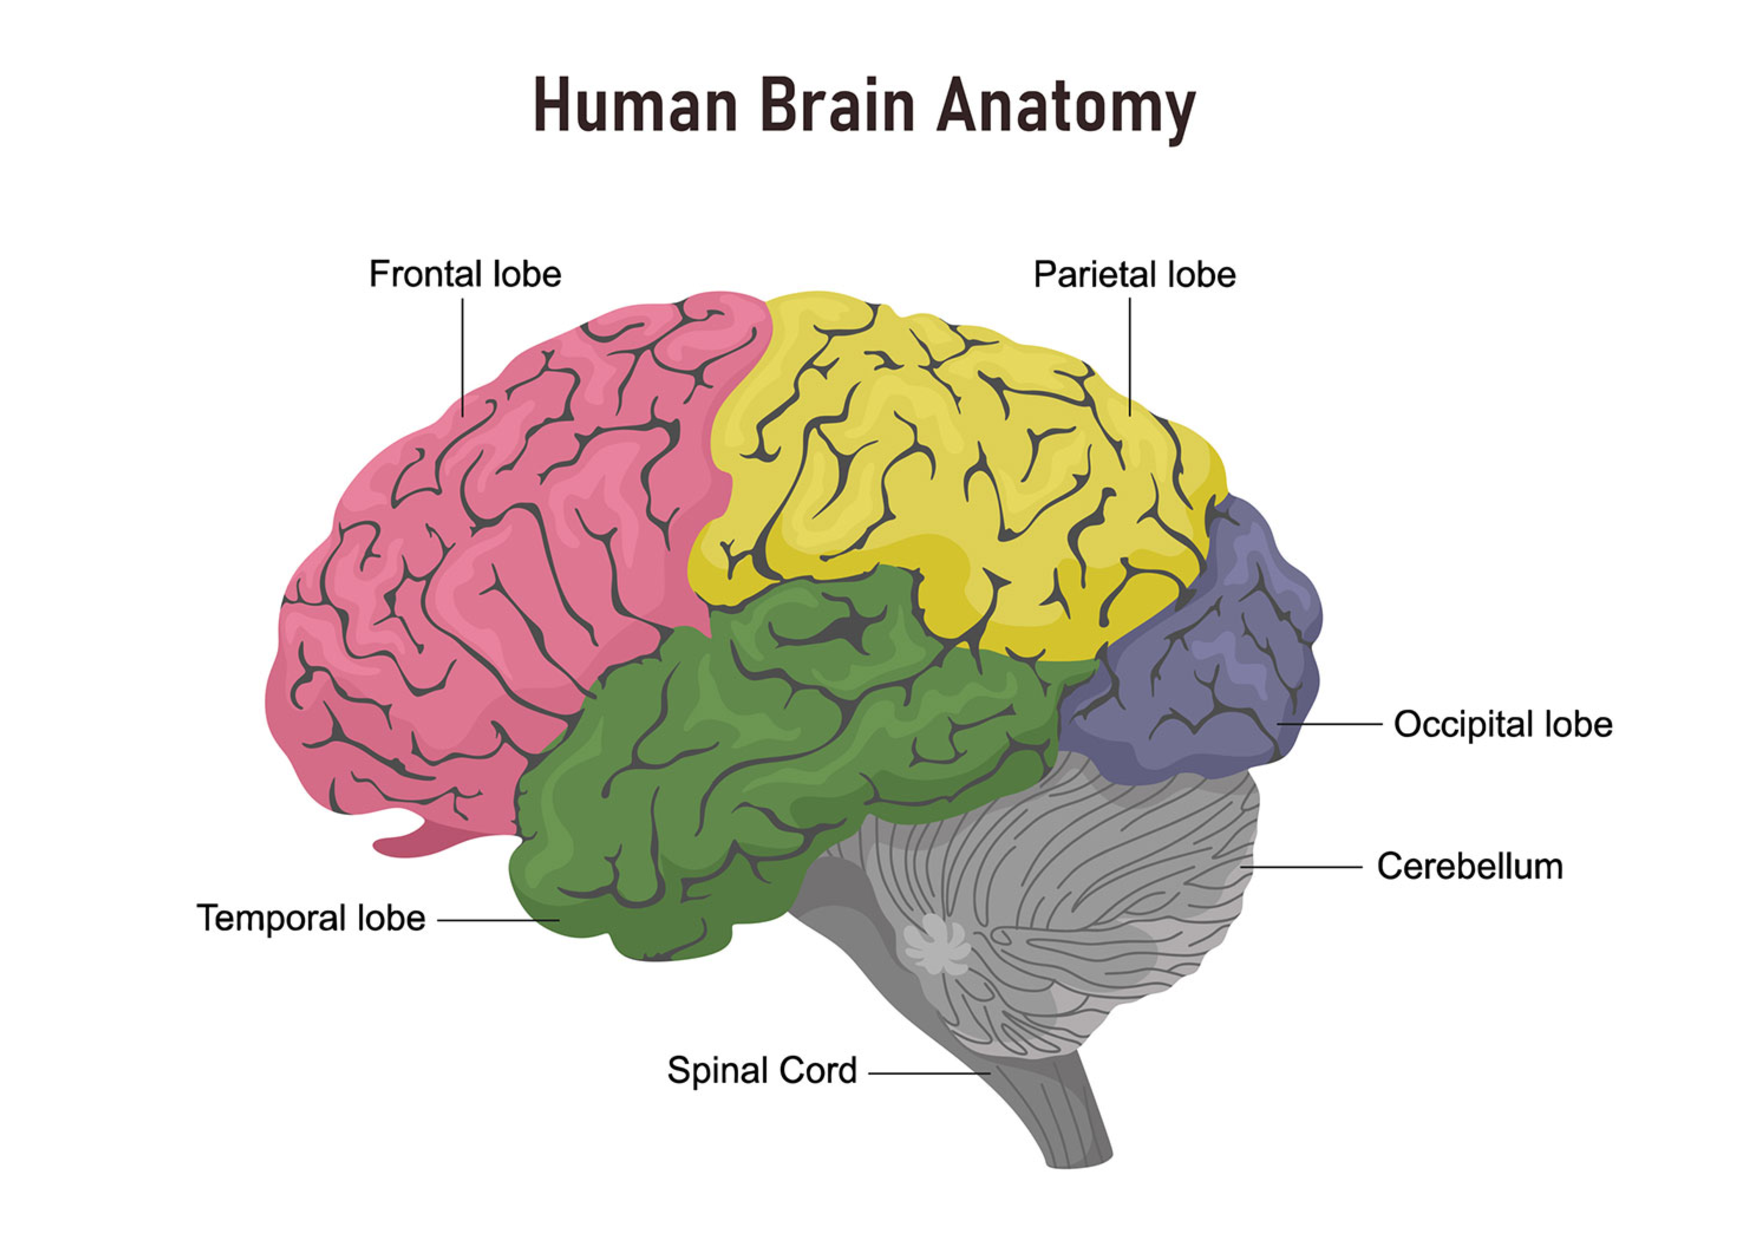
\includegraphics[width=0.7\linewidth]{Figures/Example1} 

}

\caption{Figure example. This is how we include a figure in teh text with a caption. With fig.align, you can decide wether to left-aling, right-align or centre it relative to the page. With out.width you can plot your figure in a smaller size than its original size.}\label{fig:examplefig1}
\end{figure}

Finally, here is an example for a table (Table \ref{tab:exampletable1}).

\begin{table}[H]

\caption{\label{tab:exampletable1}Table example. With the command align you can choose how to aling each column. The next lign of code within this chunk allows you to stick the table exactly where you created it.}
\centering
\begin{tabular}[t]{l|c|c}
\hline
Numbers & Ones & Twos\\
\hline
Number 1 & 1 & 2\\
\hline
Number 2 & 1 & 2\\
\hline
\end{tabular}
\end{table}

\pagebreak

\hypertarget{chapter-2-title-of-the-chapter}{%
\section{Chapter 2: Title of the chapter}\label{chapter-2-title-of-the-chapter}}

\hypertarget{section-title-1}{%
\subsection{Section title}\label{section-title-1}}

\hypertarget{section-title-2}{%
\subsection{Section title}\label{section-title-2}}

\hypertarget{section-title-3}{%
\subsection{Section title}\label{section-title-3}}

\hypertarget{section-title-4}{%
\subsection{Section title}\label{section-title-4}}

\pagebreak

\hypertarget{chapter-3-title-of-the-chapter}{%
\section{Chapter 3: Title of the chapter}\label{chapter-3-title-of-the-chapter}}

\hypertarget{section-title-5}{%
\subsection{Section title}\label{section-title-5}}

\hypertarget{section-title-6}{%
\subsection{Section title}\label{section-title-6}}

\hypertarget{section-title-7}{%
\subsection{Section title}\label{section-title-7}}

\hypertarget{section-title-8}{%
\subsection{Section title}\label{section-title-8}}

\pagebreak

\hypertarget{chapter-4-title-of-the-chapter}{%
\section{Chapter 4: Title of the chapter}\label{chapter-4-title-of-the-chapter}}

\hypertarget{section-title-9}{%
\subsection{Section title}\label{section-title-9}}

\hypertarget{section-title-10}{%
\subsection{Section title}\label{section-title-10}}

\hypertarget{section-title-11}{%
\subsection{Section title}\label{section-title-11}}

\hypertarget{section-title-12}{%
\subsection{Section title}\label{section-title-12}}

\pagebreak

\hypertarget{chapter-5-title-of-the-chapter}{%
\section{Chapter 5: Title of the chapter}\label{chapter-5-title-of-the-chapter}}

\hypertarget{section-title-13}{%
\subsection{Section title}\label{section-title-13}}

\hypertarget{section-title-14}{%
\subsection{Section title}\label{section-title-14}}

\hypertarget{section-title-15}{%
\subsection{Section title}\label{section-title-15}}

\hypertarget{section-title-16}{%
\subsection{Section title}\label{section-title-16}}

\pagebreak
\beginsupplementAone

\hypertarget{appendix-1}{%
\section*{Appendix 1}\label{appendix-1}}
\addcontentsline{toc}{section}{Appendix 1}

Here is an example of another figure (Figure \ref{fig:examplefig2}) and another table (Table \ref{tab:exampletable2}) to show you that the numbering changed for this section.

\begin{figure}

{\centering 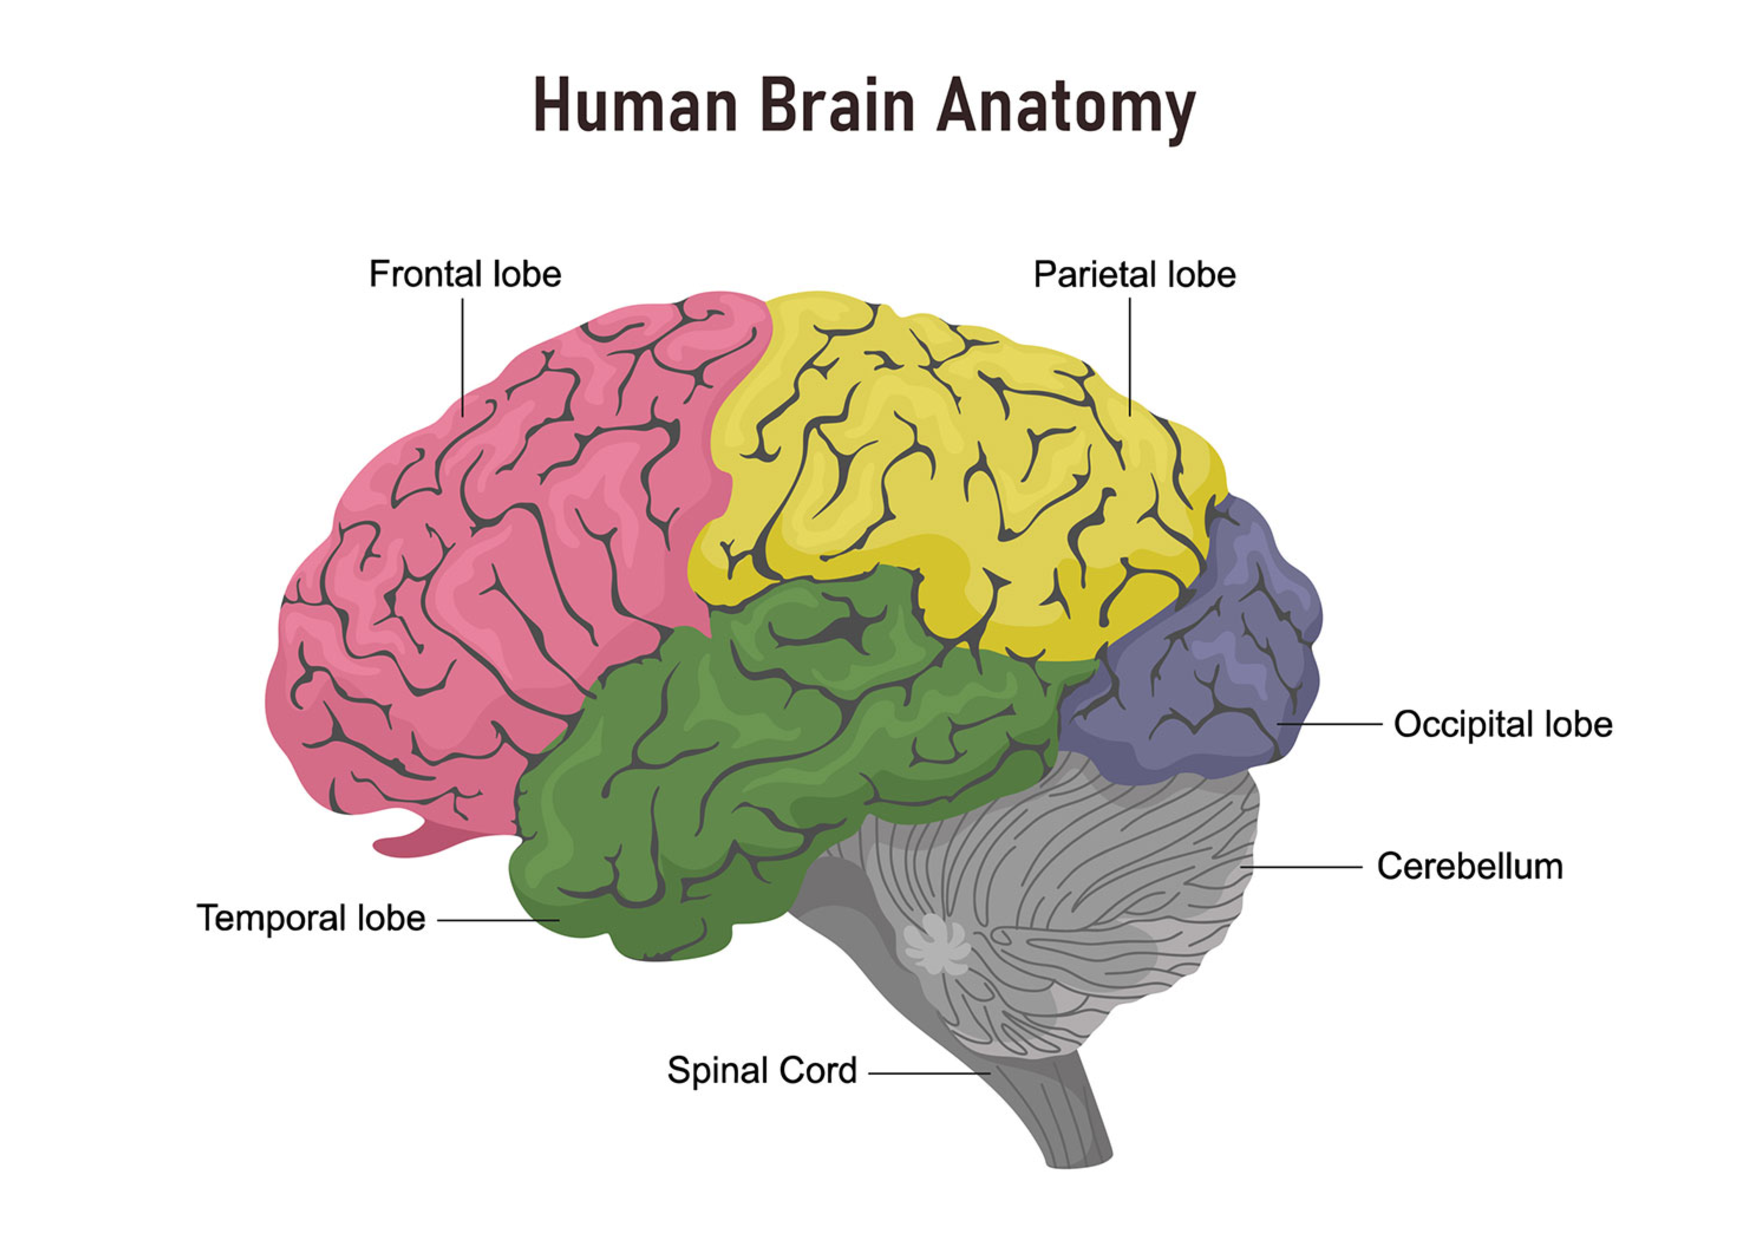
\includegraphics[width=0.8\linewidth]{Figures/Example2} 

}

\caption{Figure example for appendix. The figure count is reset for the appendix with the command used at the beginning, so this figure is the first and is set to be A1.1.}\label{fig:examplefig2}
\end{figure}

\begin{table}[H]

\caption{\label{tab:exampletable2}Table example 2. Similar to the figure count, the table count is reset and this is the first table.}
\centering
\begin{tabular}[t]{l|c|c}
\hline
Numbers & Threes & Fours\\
\hline
Number 3 & 3 & 4\\
\hline
Number 4 & 3 & 4\\
\hline
\end{tabular}
\end{table}

\pagebreak

\hypertarget{references}{%
\section*{References}\label{references}}
\addcontentsline{toc}{section}{References}

\hypertarget{refs}{}
\begin{CSLReferences}{1}{0}
\leavevmode\vadjust pre{\hypertarget{ref-Author2024}{}}%
Author N. 2024. Second example of citation. \emph{Journal that shows examples of citations}.

\leavevmode\vadjust pre{\hypertarget{ref-Author2023}{}}%
Author N. 2023. First example of citation. \emph{Journal that shows examples of citations}.

\leavevmode\vadjust pre{\hypertarget{ref-Author2025}{}}%
Author N, Authortwo N. 2025. Third example of citation. \emph{Journal that shows examples of citations}.

\leavevmode\vadjust pre{\hypertarget{ref-Author2026}{}}%
Author N, Authortwo N, Authorthree N, Authorfour N. 2026. Fourt example of citation. \emph{Journal that shows examples of citations}.

\end{CSLReferences}

\end{document}
